\documentclass[12pt,letterpaper, onecolumn]{exam}
\usepackage{amsmath}
\usepackage{amssymb}
\usepackage{sidecap}
\usepackage{tabularx}
\usepackage{csquotes}
\usepackage{makecell}
\usepackage{hyperref}
\hypersetup{
    colorlinks=true,
    linkcolor=blue,
    filecolor=magenta,      
    urlcolor=black,
    pdftitle={Overleaf Example},
    pdfpagemode=FullScreen,
}
%\usepackage[left=0.5cm,right=0.5cm,top=0.5cm,bottom=0.5cm]{geometry}
\usepackage[usestackEOL]{stackengine}
%\setstacktabbedgap{1ex} 
\usepackage{tikz}
\usetikzlibrary{decorations.pathreplacing}
\usetikzlibrary{fadings}
\def\layersep{2.5cm}

\usepackage{enumitem}
\usepackage{graphicx}
\usepackage{algorithm}
\usepackage{algpseudocode}

\usepackage{subcaption}

%\usepackage[shortlabels]{enumitem}
%\usepackage{enumerate}
\usepackage[lmargin=71pt, tmargin=0.8in]{geometry}  %For centering solution box

% \chead{\hline} % Un-comment to draw line below header
\thispagestyle{empty} 
  %For removing header/footer from page 1
\usepackage{color}
\definecolor{light-gray}{gray}{0.95}

\usepackage{listings}
\lstset{
    basicstyle=\footnotesize\ttfamily,
    escapechar=¢,
    language=python,
    frame=single,
    frameround=tttt,
    showstringspaces=false,
    backgroundcolor=\color{light-gray}
}  %For removing header/footer from page 1


\usepackage{xcolor}

\definecolor{codegreen}{rgb}{0,0.6,0}
\definecolor{codegray}{rgb}{0.5,0.5,0.5}
\definecolor{codepurple}{rgb}{0.58,0,0.82}
\definecolor{backcolour}{rgb}{0.95,0.95,0.92}

\lstdefinestyle{mystyle}{
    backgroundcolor=\color{light-gray},   
    commentstyle=\color{codegreen},
    keywordstyle=\color{magenta},
    numberstyle=\tiny\color{codegray},
    stringstyle=\color{codepurple},
    basicstyle=\ttfamily\footnotesize,
    breakatwhitespace=false,         
    breaklines=true,                 
    captionpos=b,                    
    keepspaces=true,                 
    numbers=left,                    
    numbersep=5pt,                  
    showspaces=false,                
    showstringspaces=false,
    showtabs=false,                  
    tabsize=2
}

\lstset{style=mystyle}




\begin{document}



\newtheorem{theorem}{Theorem}[section]
\newtheorem{problem}{Problem}
\newtheorem{proposition}{Proposition}[section]
\newtheorem{lemma}{Lemma}[section]
\newtheorem{corollary}[theorem]{Corollary}
\newtheorem{example}{Example}[section]
\newtheorem{definition}[problem]{Definition}

\newcommand{\BEQA}{\begin{eqnarray}}
\newcommand{\EEQA}{\end{eqnarray}}
\newcommand{\define}{\stackrel{\triangle}{=}}
\bibliographystyle{IEEEtran}
\raggedbottom
\setlength{\parindent}{0pt}
\providecommand{\mbf}{\mathbf}
\providecommand{\norm}[1]{\lVert#1\rVert}
\providecommand{\pr}[1]{\ensuremath{\Pr\left(#1\right)}}
\providecommand{\qfunc}[1]{\ensuremath{Q\left(#1\right)}}
\providecommand{\sbrak}[1]{\ensuremath{{}\left[#1\right]}}
\providecommand{\lsbrak}[1]{\ensuremath{{}\left[#1\right.}}
\providecommand{\rsbrak}[1]{\ensuremath{{}\left.#1\right]}}
\providecommand{\brak}[1]{\ensuremath{\left(#1\right)}}
\providecommand{\lbrak}[1]{\ensuremath{\left(#1\right.}}
\providecommand{\rbrak}[1]{\ensuremath{\left.#1\right)}}
\providecommand{\cbrak}[1]{\ensuremath{\left\{#1\right\}}}
\providecommand{\lcbrak}[1]{\ensuremath{\left\{#1\right.}}
\providecommand{\rcbrak}[1]{\ensuremath{\left.#1\right\}}}
\let\vec\mathbf

\newlist{mydesc}{description}{1} % create a new list called mydesc, of type "description"
\setlist[mydesc]{
  align=left, % use the align-format defined above
  leftmargin=0pt, % indentation for all the lines
  labelindent=1em, % horizontal space before label
  labelsep=0pt
   % horizontal space after label -- set to zero because we add space via "leftwithbar"
}



\begingroup  
    \centering
    
    \LARGE Weekly Report 4 - DBSCAN\\[0.5em]
    
    \large Ganji Varshitha\par
    \large AI20BTECH11009\par
\endgroup
\rule{\textwidth}{0.4pt}
\pointsdroppedatright   %Self-explanatory
\printanswers
\newcommand\Solution{
  \textbf{Solution:}\\}
\newcommand{\myvec}[1]{\ensuremath{\begin{bmatrix}#1\end{bmatrix}}}
 %Replace "Ans:" with starting keyword in solution box

\subsection*{Introduction}
\textbf{DBSCAN} stands for Density-Based Spatial Clustering of Applications with Noise.\\
It is a density based unsupervised learning algorithm which clusters data into arbitrary shape. 



\subsection*{Algorithm}
It assumes clusters are dense regions separated by regions of low density. Hence, it identifies those regions of high densities.
\subsubsection*{Key terms}
\begin{itemize}
\item \textbf{Density} : The number of points within a specific radius Eps.
\item \textbf{Epsilon or Eps} : The radius of circle around each data point to check the density.
\item \textbf{Core point} : A point is considered Core point if it has more than specific number of points(MinPts) within Eps.
\item \textbf{Border point} : A point is considered Border point if it has less than MinPts but grater than 1 point within Eps.
\item \textbf{Noise} : A point which does not have any points within Eps is considered noise.
\end{itemize}

\subsubsection*{Reachability and Connectivity}
Reachability states if a data point can be accessed from another data point directly or indirectly, whereas Connectivity states whether two data points belong to the same cluster or not.
\\In the algorithm, any points can be referred as:
\begin{itemize}
\item \textbf{Directly density reachable} : An object q is directly density-reachable from object p if q is within the $\epsilon$ Neighbourhood of p and p is a core point.
\item \textbf{Density reachable} :  An object p is density-reachable from q w.r.t $\epsilon$ and MinPts if there is a chain 
of objects $p_1,\cdots,p_n$, with $p_1 = q, p_n
= p$ such that $p_{i+1}$ is directly density-reachable 
from $p_i$ w.r.t $\epsilon$ and MinPts for all $1 \; \leq i \; \geq n$
\item \textbf{Density Connectivity} : Object p is density-connected to object q w.r.t $\epsilon$ and MinPts if there is an 
object r such that both p and q are density-reachable from r w.r.t $\epsilon$ and MinPts.
\end{itemize}

\begin{algorithm}
\caption{DBSCAN algorithm}\label{cap}
\begin{algorithmic}

\State clusterIndex = 0
\For {\text{p in dataset}}
\If{\text{p has label}}
  \State \textbf{continue}
  \EndIf
  \If{\text{neighboursCount(p,$\epsilon$) $\geq$ MinPts}}
  \State p is a core point 
  \State p.clusterId $=$ clusterIndex
  \For{neighbour in neighbours(p,$\epsilon$)}
  \If{neighbour has no clusterId}
  \State neighbour.clusterId $=$ clusterIndex
  \If{neighbour is core point}
  \State Visit all neighbours
  \EndIf
  \EndIf
  \EndFor
 	
 	\Else
 	\State p is a noise point  
  
	\EndIf
\EndFor
\State clusterIndex++


\end{algorithmic}
\end{algorithm}


\subsection*{Key points}
\begin{itemize}
\item It is density based and used euclidean distance as distance metric.
\item The algorithm is very sensitive to the parameters Epsilon(Eps) and MinPts.
\\ \textbf{Choosing MinPts}\\
Having domain knowledge is important to find MinPts. Also, its obvious that MinPts can't be 1 and should be atleast number of dimensions increased by 1.
\\ \textbf{Choosing Epsilon}:\\
This is calculated using K-distance graph which means plotting the sorted distance between a point and its Kth nearest neighbour for all points in the dataset. The distance in the graph where the maximum curvature occurs is taken as Eps.

\item The algorithm is robust to outliers
\item Algorithm does not require to specify number of clusters.
\item Algorithm may not work in high dimensional data and varying density clusters.
\end{itemize}


\subsection*{Python Implementation Example}

 
\begin{lstlisting}
class DBSCAN():
  def __init__(self,min_samples,eps,dataset):
  '''Constructor'''
    self.min_samples = min_samples
    self.eps = eps
    self.dataset = dataset
   
  
  #Auxilary functions
  def neighbours(self,pt):
    neighbours= []
    point = self.dataset[pt]
    
    for y_idx,y_pt in enumerate(self.dataset):
      norm = np.linalg.norm(y_pt - point)
      if norm <= self.eps and y_idx != pt:
        neighbours.append(y_idx)
    return neighbours

  def check_neighbours(self,pt_id,cluster_idx,cluster_to_pt):
    for neighbour in self.neighbours(pt_id):
      if cluster_to_pt[neighbour]==-1:
        cluster_to_pt[neighbour] = cluster_idx
        if len(self.neighbours(neighbour))>=self.min_samples:
          self.check_neighbours(neighbour,cluster_idx,cluster_to_pt)


  #Actual DBSCAN Code  
  def clustering(self):
    cluster_idx = 0
    #Initialising cluster indices to -1 for the whole dataset
    cluster_to_pt = [-1]*len(self.dataset)
    for pt_idx,pt in enumerate(self.dataset):
      if cluster_to_pt[pt_idx] != -1:
        continue
      if len(self.neighbours(pt_idx))>=self.min_samples:
        cluster_to_pt[pt_idx] = cluster_idx
        self.check_neighbours(pt_idx,cluster_idx,cluster_to_pt)
      cluster_idx +=1

    return cluster_to_pt 
            

\end{lstlisting}
\newpage
Running DBSCAN

\begin{lstlisting}
#Parameters: MinPts:4,Eps: 0.06
dbs = DBSCAN(4,0.06,dataset1)
p = dbs.clustering()
fig, ax = plt.subplots()

scatter = ax.scatter(dataset1[:,0],dataset1[:,1], c=p, cmap='rainbow')
legend1 = ax.legend(*scatter.legend_elements(),
                    loc="lower left", title="Cluster")
ax.add_artist(legend1)

plt.show()
\end{lstlisting}


Running K-Means using sklearn
\begin{lstlisting}
# FROM ABOVE PLOT WE HAVE OPTIMAL K = 2
kmeans = KMeans(n_clusters = 2,  random_state = 42)
label = kmeans.fit_predict(dataset1)
fig, ax = plt.subplots()

scatter = ax.scatter(dataset1[:,0],dataset1[:,1], c=label, cmap='rainbow')
legend1 = ax.legend(*scatter.legend_elements(),
                    loc="lower left", title="Cluster")
ax.add_artist(legend1)

plt.show()
\end{lstlisting}

\begin{figure}[!h]
\centering
\caption{DBSCAN Clustering}
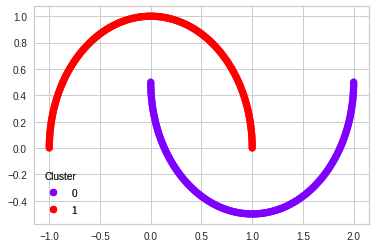
\includegraphics[width = 0.6\textwidth]{../images/DBSCAN_plot}
\end{figure}
\newpage
\begin{figure}[!h]
\centering
\caption{K-means Clustering}
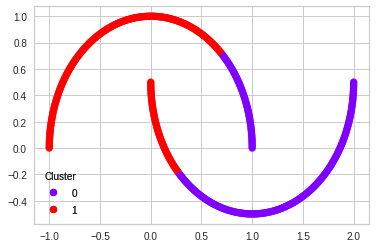
\includegraphics[width = 0.6\textwidth]{../images/K-Means_plot}
\end{figure}

\subsection*{Questions}

\begin{questions}
\question[] 
When will DBSCAN fail?
\begin{choices}
\choice For low dimensional data
\choice When density drops between clusters
\end{choices}
\begin{Solution}
B. When density drops between clusters
\end{Solution}


\question[] State the two parameters of the model.\\
\begin{Solution}
Eps and MinPts
\end{Solution}


\question[] Which of the following is false?
\begin{choices}
\choice It is sensitive to parameters
\choice We need to specify the number of clusters
\end{choices}
\begin{Solution}
B. We need to specify the number of clusters
\end{Solution}



\question[] Best case time complexity of the algorithm.\\
\begin{Solution}
If we use indexing to store the distances, time complexity turns out 
$\mathcal{O}(\text{nlogn})$
\end{Solution}



\question[] What happens if MinPts is too large?\\
\begin{Solution}
Small clusters may combine to give big cluster which ignores the small clusters.
\end{Solution}

\end{questions}


\end{document}